\documentclass{article}
\usepackage{graphicx}
\usepackage{setspace}
\usepackage{listings}
\usepackage{tikz}
\usetikzlibrary{automata,positioning,arrows.meta}
\usepackage[margin=1in]{geometry}
\usepackage{datetime}

\lstset{
language=C,
basicstyle=\footnotesize\ttfamily,
breaklines=true,
frame=single,
tabsize=2
}

\begin{document}
\begin{titlepage}
\begin{center}
{\fontsize{22}{26.4}\textbf{A Report on\ Compiler Design Lab (CS304) Mini Project}}\\
\textbf{}\\
{\textbf{Mohnish Hemanth Kumar}} (Roll No: 231CS235)\\
\vspace{0.5cm}
{\textbf{Nikhil Kottoli}} (Roll No: 231CS236)\\
\vspace{0.5cm}
{\textbf{Pal Patel}} (Roll No: 231CS240)\\
\vspace{0.3cm}
\begin{figure}[h]
{\centering {\includegraphics[height=4.5cm]{nitk_logo.png}}\par}
\end{figure}
\setstretch{2}
{\textbf{DEPARTMENT OF COMPUTER SCIENCE AND ENGINEERING}\par}
\vspace{-12pt}
{\textbf{NATIONAL INSTITUTE OF TECHNOLOGY KARNATAKA}\par}
\vspace{-12pt}
{\textbf{SURATHKAL, MANGALURU-575025}\par}
\vspace{-12pt}
{\textbf{13-August-2025}\par}
\end{center}
\pagebreak
\end{titlepage}

\tableofcontents
\newpage

\section{Overview of the Code}
The provided Lex file implements a lexical analyzer (scanner) for a subset of the C programming language. It uses Flex to define rules for recognizing tokens such as keywords, types, identifiers, numbers, strings, character literals, operators, punctuators, and preprocessor directives.  
The scanner also maintains a symbol table and constant table. The output is written to \texttt{output.md}.  
\section{Code}
Github: \texttt{https://github.com/NikhilKottoli/Compiler-Design} \\

\section{List of Recognized Tokens and Their Meaning}
\begin{itemize}
\item \textbf{PREPROC}: Preprocessor directives starting with \#.
\item \textbf{KEYWORD}: Reserved words like \texttt{if}, \texttt{for}, \texttt{while}, etc.
\item \textbf{TYPE}: Data types like \texttt{int}, \texttt{float}, etc.
\item \textbf{IDENT}: Identifiers.
\item \textbf{NUMBER}: Numeric literals.
\item \textbf{STRING}: String literals.
\item \textbf{CHAR}: Character literals.
\item \textbf{PUNCT}: Punctuation like \texttt{( ) \{ \} ;}.
\item \textbf{OP}: Operators like \texttt{+ - * /}.
\end{itemize}

\section{DFA Diagram Underlying the Scanner}
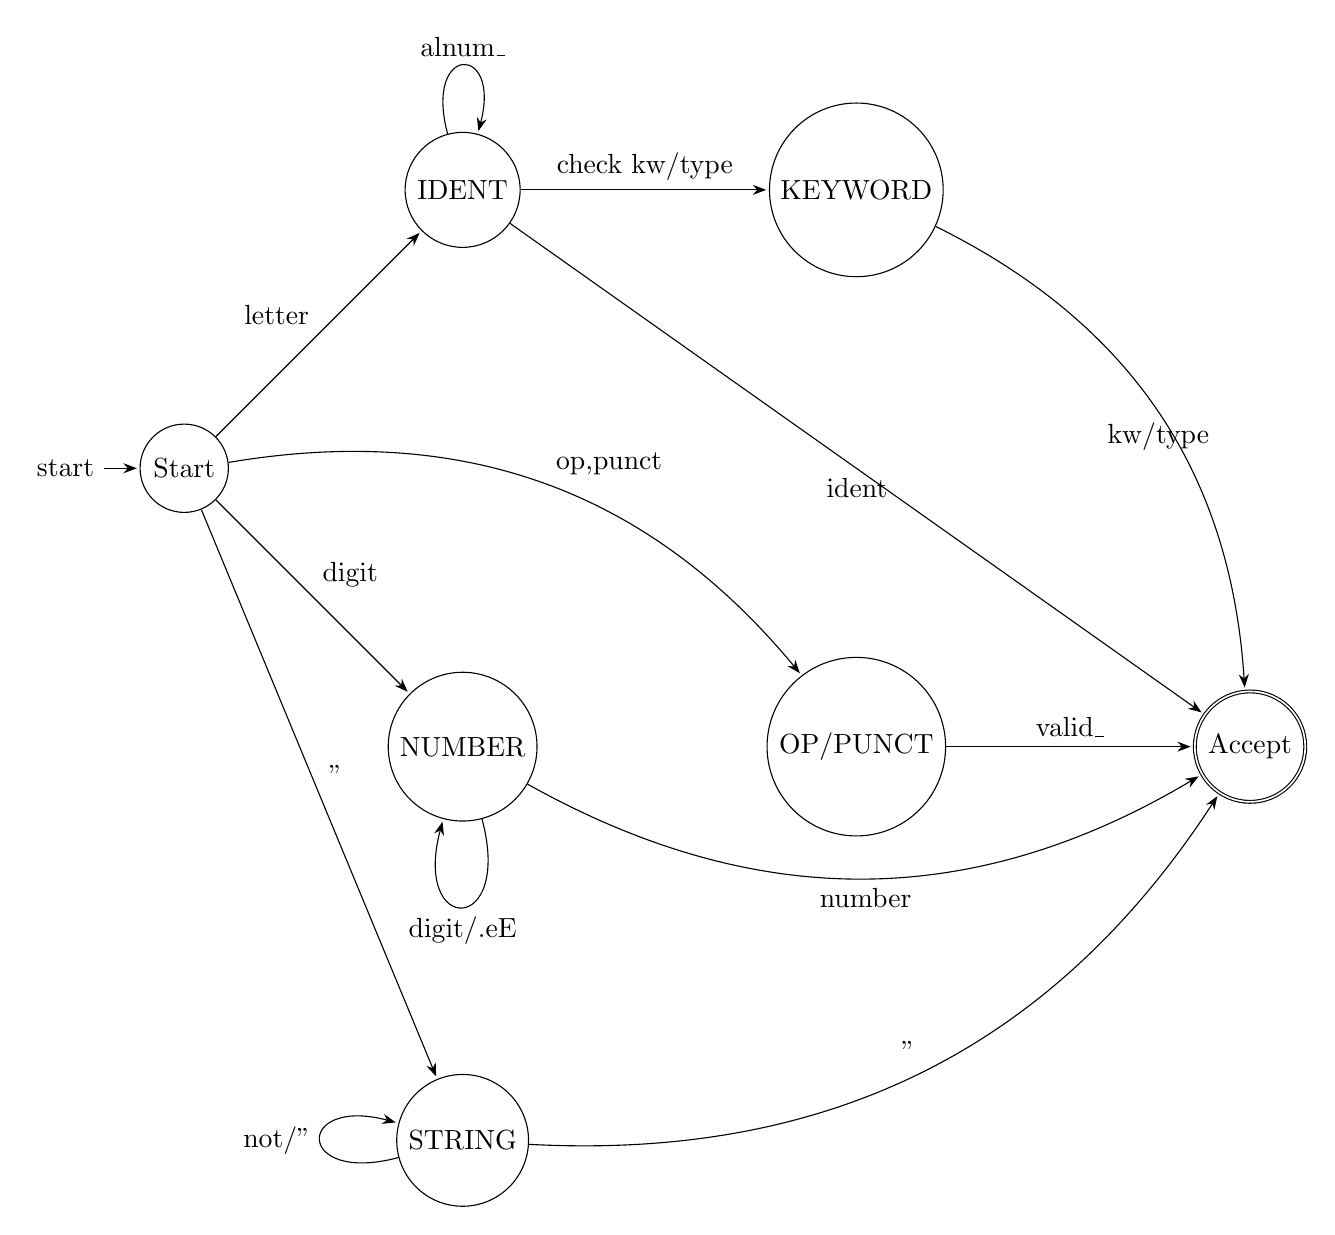
\begin{tikzpicture}[->,>=Stealth,shorten >=1pt,auto,node distance=5cm,thin]
\node[initial,state] (start) {Start};
\node[state,above right of=start] (id) {IDENT};
\node[state,below right of=start] (num) {NUMBER};
\node[state,right of=id] (kw) {KEYWORD};
\node[state,right of=num] (op) {OP/PUNCT};
\node[state,below of=num] (str) {STRING};
\node[state,accepting,right of=op] (accept) {Accept};
\path (start) edge node {letter} (id)
(start) edge node {digit} (num)
(start) edge node {"} (str)
(start) edge [bend left] node {op,punct} (op)
(id) edge [loop above] node {alnum\_} (id)
(id) edge node {check kw/type} (kw)
(num) edge [loop below] node {digit/.eE} (num)
(str) edge [bend right] node {"} (accept)
(str) edge [loop left] node {not/"} (str)
(op) edge node {valid\_} (accept)
(id) edge node [below] {ident} (accept)
(kw) edge [bend left] node [below] {kw/type} (accept)
(num) edge [bend right] node [below] {number} (accept);
\end{tikzpicture}

\section{Assumptions Made Beyond the Basic Language Description} The scanner assumes a C89/C90-like subset, without C99/C11 features like // comments in all contexts (but handles them), or complex numbers. Nested comments are supported (non-standard in C, but code handles depth). Preprocessor only handles \#define for constants; other directives are tokenized but not processed further. Identifiers in declarations capture types only on first occurrence; multi-word types (e.g., unsigned int) are concatenated. Function parameters are captured as raw strings (including types), separated by ';' for multiple calls. Array dimensions are appended only for immediate [num] after identifier in declarations. Numeric suffixes (u, l, f, etc.) are recognized but not affecting type beyond classification. No support for trigraphs or digraphs. Errors are reported for unterminated strings/chars/comments and invalid tokens, but scanning continues. Whitespace in array dimensions [ num ] is allowed.

\section{Test Cases with Results, Including Any Failures}

\subsection{Test Case 1: Simple Program}
Input:
\begin{verbatim}
int main() {
    int a = 10;
    float b = 2.5;
    char c = 'x';
    return a + b;
}
\end{verbatim}

\bigskip
\textbf{Symbol Table (excerpt):}
\begin{center}
\begin{tabular}{|l|l|l|c|l|l|}
\hline
Name & Type & Dimension & Frequency & Return Type & Parameters \\
\hline
main & int   & global & 1 & function & - \\
a    & int   & local  & 2 & variable & - \\
b    & float & local  & 3 & variable & - \\
c    & char  & local  & 4 & variable & - \\
\hline
\end{tabular}
\end{center}

\bigskip
\textbf{Constant Table (excerpt):}
\begin{center}
\begin{tabular}{|l|l|l|c|}
\hline
Name & Value & Type  & Line \\
\hline
- & 10  & int   & 2 \\
- & 2.5 & float & 3 \\
- & 'x' & char  & 4 \\
\hline
\end{tabular}
\end{center}

No errors.

\subsection{Test Case 2: With Errors}
Input:
\begin{verbatim}
int main() {
    string s = "Hello; // unterminated string
    @illegal = 5;     // invalid token
    return 0;
}
\end{verbatim}

Expected Output (excerpt):  
\begin{itemize}
\item ERROR: Unterminated string literal on Line-2
\item ERROR: Invalid token \texttt{@}  on Line-3
\end{itemize}

Failures: The scanner recovers by continuing after errors, but may misclassify subsequent tokens if states are not reset properly.

\subsection{Test Case 3: Function with Params}
Input:
\begin{verbatim}
#include <stdio.h>
#define SIZE 100
#define PI 3.14159

int area(int r, char c) {
    int arr[SIZE];
    float result = PI * arr[0] * arr[0];
    return result;
}
\end{verbatim}

\textbf{Symbol Table (excerpt):}
\begin{center}
\begin{tabular}{|l|l|l|c|l|}
\hline
Identifier & Type   & Scope  & Line & Extra Info \\
\hline
SIZE   & macro  & global & 2 & 100 \\
PI     & macro  & global & 3 & 3.14159 \\
area   & int    & global & 5 & params: (int r, char c) \\
arr    & int[]  & local  & 6 & size = SIZE \\
result & float  & local  & 7 & variable \\
\hline
\end{tabular}
\end{center}

\bigskip
\textbf{Constant Table (excerpt):}
\begin{center}
\begin{tabular}{|l|l|l|c|}
\hline
Name & Value   & Type   & Line \\
\hline
SIZE & 100     & int    & 2 \\
PI   & 3.14159 & float  & 3 \\
-    & 0       & int    & 8 \\
\hline
\end{tabular}
\end{center}

\section{Documentation on Handling Comments, Strings, and Errors} \textbf{Comments}: Single-line: "//" followed by anything until newline; ignored. Multi-line: "/" to "/", with nesting support (depth counter). If unterminated (EOF), reports "ERROR: Unterminated comment" and exits state. Handled in exclusive "comment" state to consume input without tokenizing comment \\
\\
\textbf{Strings}: Start with ", consume until " (non-escaped), supporting escapes (\textbackslash a, \textbackslash b, \textbackslash xHH, octal) and multi-line via \textbackslash\ at EOL. If newline without " reports ERROR: Unterminated string and resets to INITIAL. Exclusive "string" state with yymore() to accumulate lexeme.string Added to constants as "string". \\
\\
\textbf{Errors}: Invalid tokens: Any unmatched char triggers "ERROR: Invalid token 'char'". Unterminated constructs: Specific messages for comments, strings, chars. Output to "output.md" with line numbers; scanning continues after errors. No syntax errors (that's parser's job); only lexical. 
\end{document}
